\documentclass[a4paper,10pt]{article}
\usepackage[utf8]{inputenc}
\usepackage[T1]{fontenc}
\usepackage{lmodern}
\usepackage{graphicx}
\usepackage{tikz}
\usepackage{float}
\usepackage{longtable}
\usepackage{hyperref}
\begin{document}
\begin{titlepage}

\newcommand{\HRule}{\rule{\linewidth}{0.5mm}} % Defines a new command for the horizontal lines, change thickness here

\center % Center everything on the page
 
%----------------------------------------------------------------------------------------
%	HEADING SECTIONS
%----------------------------------------------------------------------------------------

\textsc{\LARGE Université de Mons}\\[1.5cm] % Name of your university/college
\textsc{\Large Compilation }\\[0.5cm] % Major heading such as course name

%----------------------------------------------------------------------------------------
%	TITLE SECTION
%----------------------------------------------------------------------------------------

\HRule \\[0.4cm]
{ \huge \bfseries Implémentation d'un compilateur du language \textrm{Dumbo}}\\[0.4cm] % Title of your document
\HRule \\[1.5cm]
 
%----------------------------------------------------------------------------------------
%	AUTHOR SECTION
%----------------------------------------------------------------------------------------

\begin{minipage}{0.4\textwidth}
\begin{flushleft} \large
\emph{Auteurs :}\\
Florent Delgrange \\
Clément Tamines
\end{flushleft}
\end{minipage}
~
\begin{minipage}{0.4\textwidth}
\begin{flushright} \large
\emph{Professeur:} \\
Véronique Bruyère
\emph{Assistant:} \\
Noémie Meunier
\end{flushright}
\end{minipage}\\[4cm]

% If you don't want a supervisor, uncomment the two lines below and remove the section above
%\Large \emph{Author:}\\
%John \textsc{Smith}\\[3cm] % Your name

%----------------------------------------------------------------------------------------
%	DATE SECTION
%----------------------------------------------------------------------------------------

{\large 23 mai 2016}\\[3cm] % Date, change the \today to a set date if you want to be precise

%----------------------------------------------------------------------------------------
%	LOGO SECTION
%----------------------------------------------------------------------------------------

%\includegraphics{Logo}\\[1cm] % Include a department/university logo - this will require the graphicx package
 
%----------------------------------------------------------------------------------------

\vfill % Fill the rest of the page with whitespace

\end{titlepage}

\newpage
\tableofcontents
\newpage

\section{Introduction}

Le but de ce projet est d'implémenter un compilateur pour le language \textrm{Dumbo}. Il est demandé d'adapter la grammaire fournie dans l'énoncé pour 
qu'elle gère les expressions arithmétiques, les expressions booléennes ainsi que les structures de contrôle \textbf{if} et les boucles \textbf{for}.
Ce rapport a pout but d'expliquer les techniques que nous avons utilisées afin de réaliser ce compilateur.

\section{Grammaire utilisée}
La grammaire utilisée dans ce projet est une version plus complète de la grammaire fournie dans l'énoncé :\newline
{\small
< programme > $\rightarrow$ < txt > | < txt > < programme >\\
< programme > $\rightarrow$ < dumbo\_bloc > \\
< programme > $\rightarrow$ < dumbo\_bloc > < programme > \\
< txt > $\rightarrow$ [a-zA-Z0-9; \& <> ” − .\textbackslash / \textbackslash n \textbackslash p :, ]+ \\
< dumbo\_bloc > $\rightarrow$ {{ < expressions\_list > }} \\
< expressions\_list > $\rightarrow$ < expression > ; < expressions\_list >\\
< expressions\_list > $\rightarrow$ < expression > ; \\
< expression > $\rightarrow$ print < string\_expression > \\
< expression > $\rightarrow$ for < variable > in < string\_list > do < expressions\_list > endfor \\
< expression > $\rightarrow$ for < variable > in < variable > do < expressions\_list > endfor \\
< expression > $\rightarrow$ if < boolean\_expression > do < expression\_list > endif\\
< expression > $\rightarrow$ < variable > := < string\_expression > \\
< expression > $\rightarrow$ < variable > := < string\_list > \\
< expression > $\rightarrow$ < variable > := < operation > \\
< operation > $\rightarrow$ < integer > \\
< operation > $\rightarrow$ < variable > \\
< operation > $\rightarrow$ < operation > + < operation >\\
< operation > $\rightarrow$ < operation > - < operation >\\
< operation > $\rightarrow$ < operation > * < operation >\\
< operation > $\rightarrow$ < operation > / < operation >\\
< string\_expression > $\rightarrow$ < string > \\
< string\_expression > $\rightarrow$ < variable > \\
< string\_expression > $\rightarrow$ < string\_expression > . < string\_expression > \\
< string\_list > $\rightarrow$ ( < string\_list\_interior > ) \\
< string\_list\_interior > $\rightarrow$ < string >\\
< string\_list\_interior > $\rightarrow$ < string >, < string\_list\_interior > \\
< boolean\_expression > $\rightarrow$ < boolean > \\
< boolean\_expression > $\rightarrow$ < boolean\_expression > and < boolean\_expression > \\
< boolean\_expression > $\rightarrow$ < boolean\_expression > or < boolean\_expression > \\
< boolean\_expression > $\rightarrow$ < variable > < < variable >\\
< boolean\_expression > $\rightarrow$ < variable > > < variable >\\
< boolean\_expression > $\rightarrow$ < variable > = < variable >\\
< boolean\_expression > $\rightarrow$ < variable > != < variable >\\
< boolean > $\rightarrow$ [true|false]\\
< integer > $\rightarrow$ \textbackslash d+\\
< variable > $\rightarrow$ [a-z|A-Z]+[a-z|A-Z|0-9\_]*\\
< string > $\rightarrow$ '[a-zA-Z0-9; \& <> ” − .\textbackslash / \textbackslash n\textbackslash p :, =]+' \\
}
Nous avons tout d'abord  ajoutés les opérations qui permettent de traiter des opérations arithmétiques sur des entiers ou des variables contenant des entiers et 
stocker le résultat dans une variable. Nous avons aussi ajoutés les expressions booléennes qui permettent le and et le or ainsi que des booléens qui permettent de co
comaprer des entiers contenus dans des variables. Ces booléens sont utilisés pour la structure de contreol if et doivent être mis tel qu'ils sont et non dans 
des variables.
\section{Gestion du \textbf{if} et \textbf{for}}
Le if a été implémenté via la règle < expression > $\rightarrow$ if < boolean\_expression > do < expression\_list > endif \\
La détection du mot clé if commence la détection de cette règle, nous détectons ensuite une expression booléenne et effections ensuite des expressions. Ceci
est géré dans l'arbre par un noeud spécial créé lors de la détection de cette règle. Celui-ci vérifie d'abord si la condition est vérifiée (l'expression correspond d
directement à du code python) si c'est le cas, le corps sera exécuté via le noeud correspondant nous récupérons le résultat de son exécution et l'ajoutons.
Si ce n'est pas le cas alors nous n'affichons rien. L'utilisation de noeuds gérant les différents aspects permet une gestion intuitive de ces structures. En effet,
voici le code correspondant à :
\begin{verbatim}

class IfNode():
   def __init__(self, *args):
      self.sons = args
         
   def ex(self):
      condition = self.sons[0]
      action = self.sons[1]

      res = ""
      if(condition.ex()):
         res += str(action.ex())
      return res
 
\end{verbatim}
L'éxécution de ce noeud vérifie si l'éxécution du noeud correspondant à l'expression booléenne est vraie, si c'est le cas il exécute le noeud correspondant à
la condition, sinon il retourne une chaine vide (ce qui est équivalent à ne rien retourner).

Le for se fait de la même façon, nous prenons en paramètre une condition 
\begin{verbatim}
 class ForNode():
   def __init__(self, *args):
      self.sons = args
         
   def ex(self):
      var_name = str(self.sons[0]) #Nom de la variable

      initial_value = "" #Valeur initiale de la variable

      #Si la variable éxiste déjà et a une valeur, nous la retenons
      if var_name in variables:
         initial_value = variables[var_name]

      list_or_var = self.sons[1].ex() #Récupérons le contenu de la var ou de la liste
      
      action = self.sons[2]
      res = ""
      for var in list_or_var:
         variables[var_name] = var
         res+=action.ex()

      #Si la variable avait une valeur initiale, nous la réinstallons
      if initial_value != "":
         variables[var_name] = initial_value

      return res
\end{verbatim}

Nous vérifions d'abord si la varable utilisée dans le for est une variable déjà initialisée quelque part. Il est important que cette variable garde sa valeur
initiale à la fin de l'éxécution de la boucle. Nous nous occupons donc de retenir la valeur initiale si elle éxiste. Nous récupérons ensuite le contenu de la 
variable qui est une liste ou bien directement une liste via l'exécution du noeud correspondant. Pour chaque élément de la liste, nous affectons sa valeur à la variable
temporaire dans notre liste globale de variables et exécutons ensuite le corps de la via acction.ex(). Nous ajoutons le résultat à une chaine de caractère qui
sera renvoyée à la fin de l'exécution du noeud.

\section{Difficultés rencontrées}
Lorceque nous avons débutés ce projet, nous avons mis du temps à comprendre que l'analyseur syntxique construisait l'arbre de dérivation et l'écutait au fur 
et à mesure dans les exemples des Tps. Nous nous sommes alors rendus compte que nous dervions implémenter une structure de donnée avec des noeuds portant différentes
fonctions pour exécuter le code et remonter à la racine de l'arbre les valeurs
\subsection{Mauvaise détection des lexèmes}
Nous nous sommes rendu compte qu'il nous faudrait deux états, l'un pour détecter des lexèmes lorsque nous étions hors d'un dumbo bloc contenant du code et l'autre
lorsque nous étions dans un dumbo bloc. Nous avons appellés cet état inBlock. Hors de cet état, juste du etxte peut être détecté. Un noeud texte contient alors la chaine
de caractère associée. Lorsque deux {{ sont rencontrés, nous entrons dans l'état inBlock et les mots clés ainsi que variables peuvent êter détectés. Le
compilateur ne confondra pas le TXT avec des noms de varaibles puisque chacun de ces lexèmes appartient à un état différent et le compilateur peut alors les 
diféfrecier selon l'état dans lequel il se trouve. Dans l'état inBlock nous avons remarqués que les symboles réservés du languages ainsi que les nombres entiers 
étaient détectés comme des noms de variables. En effet le lexème variale étant le premier, lorsque le compilateur rencontre un if, celui-ci était détecté comme 
une vriable et rendait l'exécution impossible. Il en est de même pour or, and, ect. Nous avons réglés ce problème avec un dictionnaire de mots clés réservés.
Lorsque if est détecté comme une variable, le dictionnaire est consulté, if faisant partie du dictionnaire de mots clé, et le type correspond à if dans ce ditonaire
étant IF, la valeur du lexème est modifiée. En ce qui concerne les nombres entiers, nous avons empéchés les noms de variables de commencer par un entier, comme cela
se fait dans de nombreux autres languages ce qui enlèves l'ambiguité entre les nombres entiers et les variables.
\subsection{Création et parcours de l'arbre}
Lors de l'analyse syntaxique, l'arbre de dérivation est créé. Chaque règle de la grammaire crée un noeud spécial et ces noeuds ont eux mêmes des fils. La racine 
de l'arbre ainsi créé est retourné lorsque l'analyse syntaxique est terminée. Il ne nous reste plus qu'à demander l'exécution de l'arbre qui se fait en appellant
la méthode \textrm{ex()} sur la racine. Celui-ci va alors récursivement appeller cette méthode sur ces fils et récupérer le résultat de cette exécution qui sera le
résultat de l'exécution du programme. Nous avons illustré ce principe via l'exemple de programme suivant : \\
programme : dumbobloc programme
p[0] = RegularNode(p[1],p[2])

\subsection{Mode d'emplois}
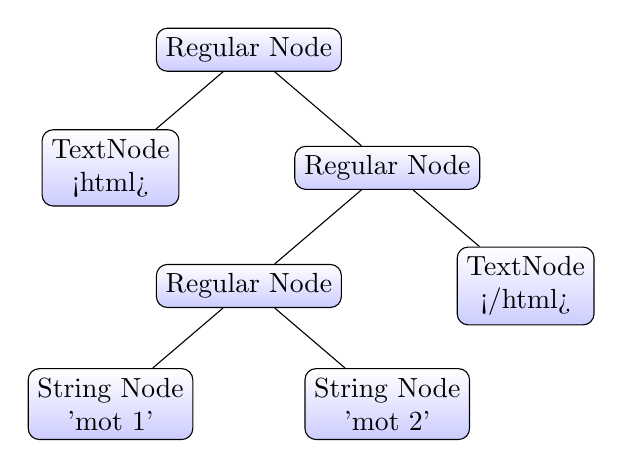
\begin{tikzpicture}[sibling distance=10em,
  every node/.style = {shape=rectangle, rounded corners,
    draw, align=center,
    top color=white, bottom color=blue!20}]]
    \node {Regular Node}
    child { node  {TextNode \\ <html>} }
    child{ node {Regular Node}
        child { node {Regular Node}
            child { node{String Node \\ 'mot 1'} }
            child { node{String Node \\ 'mot 2'} }
        }
        child { node{TextNode \\ </html>} }
    };
\end{tikzpicture}

\end{document}
